\documentclass{article}
\usepackage{cmap}
\usepackage[T2A]{fontenc}
\usepackage[utf8]{inputenc}
\usepackage[english,russian]{babel}
\usepackage{setspace}
\usepackage{geometry}
\usepackage{graphicx}
\usepackage{amsfonts}
\usepackage{amsmath}
\graphicspath{{graphicslab3/}}
\DeclareGraphicsExtensions{.pdf, .png, .jpg, .fig}
\geometry{top=2cm}
\geometry{bottom=2cm}
\geometry{left=2cm} % отступ справа
\geometry{right=2cm} % отступ слева

\begin{document}
	\begin{center}
		\hfill \break
		\begin{center}
			\huge{Санкт-Петербургский политехнический университет\\
				Высшая школа прикладной математики\\
				и вычислительной физики, ФизМех}
		\end{center}
		\hfill \break
		\hfill \break
		\hfill \break
		\hfill \break
		\hfill \break
		\huge{Направление подготовки\\
			«Прикладная математика и информатика»}\\
		\hfill \break
		\hfill \break
		\hfill \break
		\hfill \break
		\hfill \break
		\hfill \break
		\fontsize{14pt}{14pt}\selectfont
		Отчет по лабораторной работе №3\\
		«Численное интегрирование обобщенными квадратурными формулами Ньютона-Котеса»\\
		\hfill \break
		\hfill \break
		\hfill \break
		\hfill \break
		\hfill \break
	\end{center}
	\hfill \break
	\hfill \break
	\fontsize{12pt}{12pt}\selectfont
	\begin{tabular}{cccc}
		\hspace{1cm}Выполнил студент гр. 5030102/00003 & {\hspace{3cm}} & & Петрошенко А.В. \\\\
		\hspace{-3cm}Преподаватель: &{\hspace{1cm}}& & {\hspace{1cm}} Курц В.В. \\\\
	\end{tabular}\\
	\hfill \break
	\hfill \break
	\hfill \break
	\hfill \break
	\hfill \break
	\hfill \break
	\begin{center} Санкт-Петербург\\ 
		2021\\
	\end{center}
	\thispagestyle{empty}
	\newpage
	\begin{center} \textbf{Формулировка задачи и ее формализация}\end{center}
	Задача нахождения значения определенного интеграла на некотором промежутке очень часто встречается во всех технических областях науки. Существует множество способов интегрирования различных функций. Зачем же нужно тогда численное интегрирование?
	\begin{enumerate}
		\item Некоторые функции не поддаются интегрированию ни одним из известных способов
		\item Численный метод быстрее, если функция достаточно сложная для ручного интегрирования
	\end{enumerate}
	\underline{Постановка задачи:}\\
	Представим определённый интеграл на промежутке $[a,b]$ функции $F(x)$ в виде
	\begin{equation}
		\int\limits_{a}^{b}F(x)dx = \int\limits_{a}^{b}p(x)f(x)dx
	\end{equation}
	Формулы вида
	\begin{equation}
		\int\limits_{a}^{b}p(x)f(x)dx \approx \sum_{k=1}^{n}A_kf(x_k)
	\end{equation}
	называются квадратурными формулами.\\
	$A_k$ и $x_k \in [a,b]$ - коэффициенты и узлы квадратурной формулы.\\
	\\
	Число $m$ называется алгебраическим порядком точности квадратурной формулы (2), если 
	\begin{enumerate}
		\item квадратурная формула точна для всех полиномов степени $m$ и ниже
		\item существует хотя бы один полином степени $m+1$, для которого она не точна.
	\end{enumerate}
	Условия на весовую функцию $p(x)$
	\begin{enumerate}
		\item $p(x) \geq 0, \forall x \in [a,b]$
		\item $c_k = \int\limits_{a}^{b}p(x)x^kdx < \infty$
	\end{enumerate}
	Если алгебраический порядок точночти равен $m$, то
	\begin{equation}
		\begin{cases}
			A_1+A_2+...A_n = c_0\\
			A_1x_1+A_2x_2+...+A_nx_n = c_1\\
			... = ...\\
			A_1x_1^m+A_2x_2^m+...+A_nx_n^m = c_m
		\end{cases}
	\end{equation}
	Из данной системы уравнений мы можем выделить 3 вида квадратурных формул:
	\begin{enumerate}
		\item Узлы и коэффициенты не фиксируются, тогда гарантированный алгебраический порядок точности равен $2n-1$\\
		Квадратурные формулы Гаусса
		\item Все узлы $x_i$ заданы и различны, тогда гарантированный алгебраический порядок точности равен $n-1$\\ 
		Квадратурные формулы интерполяционного типа
		\item Зафиксировано $r$ параметров, $0<r<n$, тогда гарантированный алгебраический порядок точности равен $2n-1-r$\\
		Квадратурные формулы смешанного типа
	\end{enumerate}
	В данной работе будет реализована квадратурная формула интерполяционного типа.\\
	\\
	Таким образом, нужно найти все коэффициенты $A_k$, подставить их в формулу (2), и найти значение интеграла.
	\begin{center} \textbf{Алгоритм метода и условия его применимости}\end{center}
	Мы рассматриваем квадратурные формулы Ньютона-Котеса, для которых выполнены условия:
	\begin{enumerate}
		\item $p(x) \equiv 1$
		\item $x_k = a + h(k-1), h = \frac{b-a}{n-1}$
	\end{enumerate}
	Так как нам задана табличная функция, то мы можем построить интерполяционный полином Лагранжа:
	\begin{equation}
		L_{n-1}(x) = \sum_{k=1}^{n}f(x_k)\Phi_k(x_k)
	\end{equation}
	Отсюда видно, что 
	\begin{equation}
		A_k = \int\limits_{a}^{b}\Phi_k(x)dx, \Phi_k(x) = \prod_{j=1, j\neq k}^{n}\frac{x-x_j}{x_k-x_j}
	\end{equation}
	$x=a+th, t \in [0, n-1] \Rightarrow$\\
	$x-x_j = h(t-j+1), x_k-x_j = h(k - j)$\\
	$A_k = h\int\limits_{0}^{n-1}\prod\limits_{j=1, j\neq k}^{n}\frac{t-j+1}{k-j}dt$\\
	$\overline{\omega}(t) = \prod\limits_{j=0}^{n-1}(t-j)$\\
	Тогда мы получаем, что
	\begin{equation}
		A_k=h\int\limits_{0}^{n-1}\frac{\overline{\omega}(t)}{t-k+1}\frac{dt}{(k-1)(k-2)...(1)(-1)(-(n-k))} =  h\frac{(-1)^{n-k}}{(k-1)!(n-k)!} \int\limits_{0}^{n-1}\frac{\overline{\omega}(t)}{t-k+1} = hH_n^{(k)}
	\end{equation}
	$H_n^{(k)}$ - коэффициенты Ньютона-Котеса\\
	\\
	\underline{Формула 3/8, $n=4$}\\
	$h = \frac{b-a}{3}, x_1 = a, x_2 = a+h, x_3 = a+2h, x_4 = a+3h$
	\begin{equation}
		\int\limits_{a}^{b}f(x)dx \approx \frac{3h}{8}(f(a) + 3f(a+h)+ 3f(a+2h)+ f(a+3h)) = S_4(f)
	\end{equation}
	То есть $H_4^{(1)} = H_4^{(4)} = \frac{3}{8}, H_4^{(2)} = H_4^{(3)} = \frac{9}{8}$\\
	Остаточный член
	\begin{equation}
		R_4(f) = -\frac{3h^5}{80}f^{(IV)}(\eta)
	\end{equation}
	\\
	\underline{Обобщенная формула:}\\
	Разобъем отрезок $[a,b]$ на $3N$ интервалов длиной $h = \frac{b-a}{3N}$
	\begin{equation}
		S_{4, N}(f) = \frac{3h}{8}(f(a) + f(b) + 3\sum_{k=1}^{N}(f(x_{3k-2}) + f(x_{3k-1})) + 2\sum_{k=1}^{N-1}f(x_{3k}))
	\end{equation}
	Остаточный член
	\begin{equation}
		R_{4, N}(f) = \sum_{k=1}^{N}-\frac{3h^5}{80}f^{(IV)}(\eta_k) = -\frac{3h^5}{80}N\underbrace{\frac{1}{N}\sum_{k=1}^{N}f^{(IV)}(\eta_k)}_{f^{(IV)}(\eta)} = -\frac{h^4}{80}(b-a)f^{(IV)}(\eta)
	\end{equation}
	\underline{Условия применимости:}\\
	\begin{enumerate}
		\item Как уже было сказано ранее узлы сетки должны быть различны, что выполняется за счет реализации равномерной сетки.
	\end{enumerate}
	\begin{center} \textbf{Предварительный анализ задачи}\end{center}
	В данной работе будет рассматриваться функция $f(x) = 0.5^x + 1 - (x-2)^2$. Она бесконечно дифференцируема, следовательно имеет четвертую производную на $[a,b]$.
	\begin{center} \textbf{Тестовый пример для задач малой размерности}\end{center}
	$$f(x) = 0.5^x + 1 - (x-2)^2, a = -6, b = 6$$
	$$\int f(x)dx = F(x) = \frac{0.5^x}{ln(0.5)} + x - \frac{(x-2)^3}{3} + C$$
	$$\int\limits_a^bf(x)dx = F(b) - F(a) = -87.69$$
	\underline{1 разбиение:}\\
	$$h = \frac{b-a}{3} = 4$$
	\begin{center}
		\begin{tabular}{|c|c|c|c|c|}
			\hline
			$x_i$ & -6 & -2 & 2 & 6 \\ 
			\hline
		\end{tabular}
	\end{center}
	$$S_{4, 1}(f) = \frac{3*4}{8}(1 - 11 + 1.25 - 15) = -64.85$$
	Фактическая погрешность $\epsilon = 22.84$\\
	\underline{2 разбиения:}\\
	$$h = \frac{b-a}{6} = 2$$
	\begin{center}
		\begin{tabular}{|c|c|c|c|c|c|c|c|}
			\hline
			$x_i$ & -6 & -4 & -2 & 0 & 2 & 4 & 6 \\ 
			\hline
		\end{tabular}
	\end{center}
	$$S_{4, 2}(f) = \frac{3*4}{8}((1 - 19 - 11 - 2) + (-2 + 1.25 - 2.93 - 15)) = -84.78$$
	Правило Рунге:
	$$\frac{|S_{4, 2}(f) - S_{4, 1}(f)|}{2^m - 1} = \frac{84.78-64.85}{15} = 1.33$$
	Фактическая погрешность $\epsilon = 2.91 > 1.33$\\
	\underline{4 разбиения:}\\
	$$h = \frac{b-a}{12} = 1$$
	\begin{center}
		\begin{tabular}{|c|c|c|c|c|c|c|c|c|c|c|c|c|}
			\hline
			$x_i$ & -6 & -5 & -3 & -2 & -1 & 0 & 1 & 2 & 3 & 4 & 5 & 6 \\
			\hline
		\end{tabular}
	\end{center}
	$$S_{4, 4}(f) = \frac{3*4}{8}((1 - 16 - 19 - 16) + (-16 - 11 - 6 - 2) + (-2 + 0.5 + 1.25 + 0.125) + (0.125 - 2.93 - 7.97 - 15)) = -87.45$$
	Правило Рунге:
	$$\frac{|S_{4, 4}(f) - S_{4, 2}(f)|}{2^m - 1} = \frac{87.45-84.78}{15} = 0.178$$
	Фактическая погрешность $\epsilon = 0.24 > 0.178$\\
	\\
	Из результатов видно, что погрешность с каждым разбиением уменьшилась на порядок
	\begin{center} \textbf{Контрольные тесты}\end{center}
	\begin{enumerate}
		\item Зададим равномерную сетку и посчитаем интеграл с различной точностью, меняя ее от $0.1$ до $10^{-14}$.
	\end{enumerate}
	\begin{center} \textbf{Модульная структура программы}\end{center}
	\verb|double f(double x)|
	- сама функция.\\
	\\
	\verb|double Integrate(double h, double a, int n)|\\
	\verb|pair<double, int> Newton_Cotes(double a, double b, double eps)|\\
	- Реализация формулы 3/8.
	\begin{center} \textbf{Численный анализ}\end{center}
	$\triangleright$ \underline{Погрешность:}\\
	\begin{center} 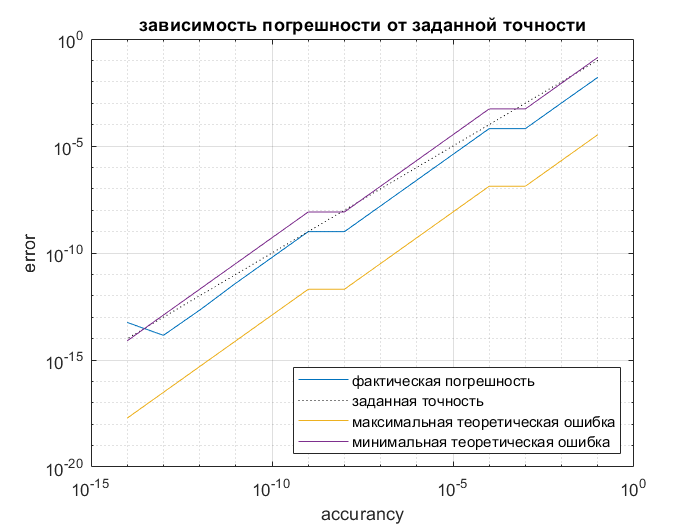
\includegraphics[scale = 0.7]{Погрешность} \end{center}
	Из графика видно, что все заданные точности достигаются, за исключением последней точки, что связано с ограниченной точностью типа данных double в языке C++.\\
	\newpage
	$\triangleright$ \underline{Количество разбиений:}\\
	\begin{center} 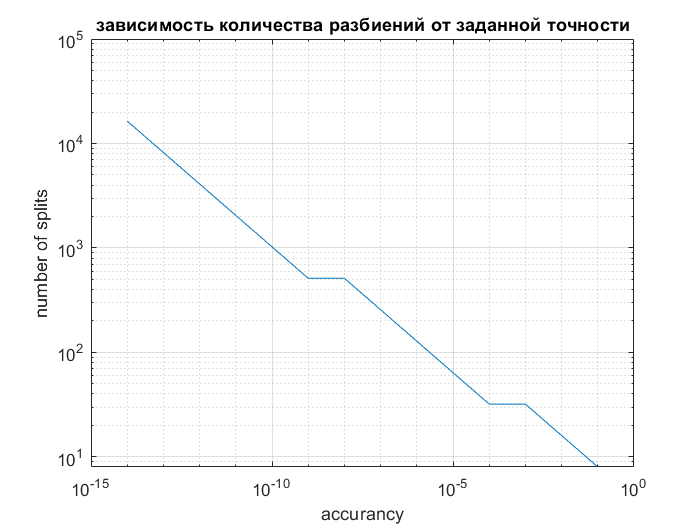
\includegraphics[scale = 0.7]{Количество разбиений} \end{center}
	По графику видно, что зависимость линейная и количество разбиений почти каждый раз растет в 2 раза.
	\begin{center} \textbf{Общие выводы}\end{center}
	В данной лабораторной работе мы научились численно вычислять опредленный интеграл на заданном промежутке с помощью формулы Ньютона-Котеса для 4х точек(3/8). Реализация метода очень простая, что видно из модульной структуры. Метод довольно эффективный, но он проигрывает формуле Симпсона, где алгебраический порядок точности такой же, но вычислений меньше. 
\end{document}